\subsection{Wyniki dla podziału na $m \cdot k$ obszarów}

Ten podrozdział opisuje wyniki podziału siatki dla $m$ node'ów, każdy z nich zawierający $k$ rdzeni.
Celem jest otrzymanie $m \cdot k$ maksymalnie równych pod względem pola partycji oraz minimalizacja długości granic
między nimi.
\subsubsection{Wyniki dla podziału siatek bez obszarów niepodzielnych i wyłączonych z obliczeń}
Dla tej kategorii kryterium zawsze była długość granic.
Na rysunku \ref{result:w1} widzimy partycjonowanie siatki $100$x$100$ bez obszarów wyłączonych z obliczeń oraz
niepodzielnych.
Rezultat w kwestii długości granic jest bardzo dobry w porównaniu do innych bibliotek, które znajduje się na rysunku
\ref{im:partitioning_results}.
\begin{figure}[h]
\centering
\begin{subfigure}{.5\textwidth}
    \centering
    \fbox{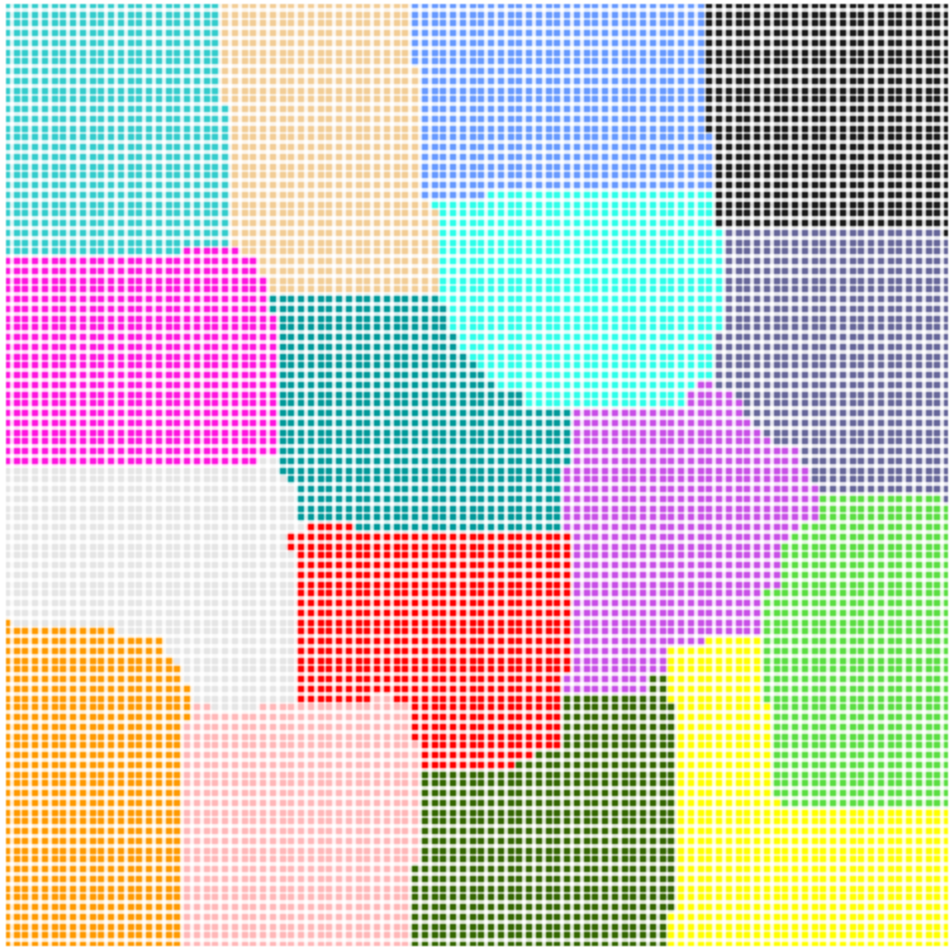
\includegraphics[width=0.8\linewidth]{images/results/m_k/without/1/partitioning}}
    \caption[short]{}
\end{subfigure}%
\begin{subfigure}{.5\textwidth}
    \centering
    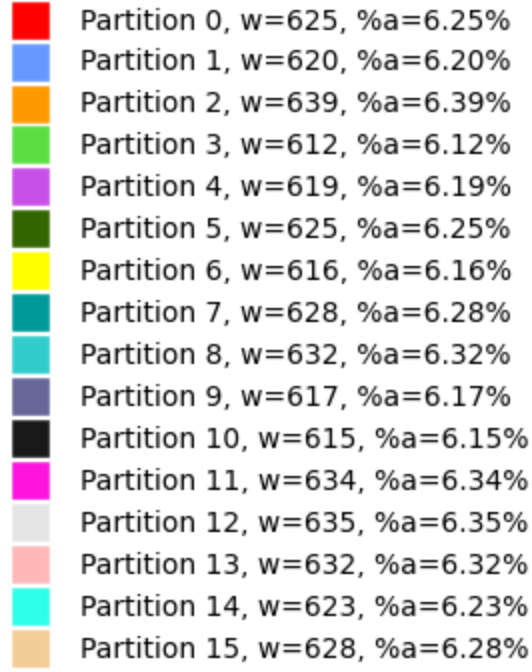
\includegraphics[width=0.6\linewidth]{images/results/m_k/without/1/results}
    \caption[short]{}
\end{subfigure}
\caption{Siatka $100$x$100$. Podział na $16$ partycji. Sumaryczna długość granic dla tego wyniku wynosi $686$.
Wybór najlepszego rezultatu wedle kryterium najmniejszej długości granic. }
\label{result:w1}
\end{figure}
Wszystkie te biblioteki traktowane są przez literature jako biblioteki dające wyniki state-of-the-art.
Z wynikiem $686$ metoda przedstawiona w tej pracy plasuje się blisko biblioteki Jostle i Metis,
które otrzymały odpowiednio $695$ oraz $688$.
Metoda zaprezentowana w niniejszej pracy bazuje na metodzie używanej przez bibliotekę Party, która dla tego problemu
otrzymuje wynik $615$.
Jest to wynik niemal idealny.
Wynikiem idealnym dla długości granic byłby wynik $600$.
Charakterystyką tego podziału jest to, że ze względu na brak obszarów niepodzielnych, które mogą utrudniać
wymianę granicznych wierzchołków udało się otrzymać niemal idealnie równe pola.
Ciężko powiedzieć, czemu jest aż tak duża różnica w stosunku do biblioteki Party.
Być może przesądziły o tym różnice w implementacji, które najprawdopodobniej wyniknęły z nie dość szczegółowo opisanego algorytmu
w artykule dotyczącym biblioteki Party \cite{1364754}.
Przyglądając się mojemu rezultatowi, można zaproponować kilka pomniejszych usprawnień, które mogłyby jeszcze trochę polepszyć wynik.
Można by przykładowo kosztem wielkości pól, zmusić algorytm do tworzenia prostych granic między obszarami.
Ciężko mi jednak wyobrazić sobie modyfikację, która sprawiałaby, że obszary ustawiałyby się tak jakby siatka dzielona
była pionowymi i poziomymi separatorami w algorytmie, który ma charakterystykę losową.
Musi wydarzyć się naprawdę duży zbieg okoliczności, aby nastąpił taki podział.
W jakiś sposób jest to możliwe dla biblioteki \cite{1364754}.
W związku powyższym wnioskuję, że w algorytmie biblioteki Party \cite{1364754} muszą być jeszcze jakieś dodatkowe
różnice względem rozwiązań opisanych w artykule.
Kolejną różnicą jest czas wykonania partycjonowania, który dla sprzętu wyposażonego w Pentium III $933$ MHz dual processor
wraz z $1$ GB pamięci operacyjnej dla Party wyniósł $0.03$s.
Dla mojego sprzętu wyposażonego w $2.3$ GHz Quad-Core Intel Core i$5$ z $2018$ roku wraz z $8$ GB pamięci operacyjnej
czas ten wyniósł $18$s.
Jest to o tyle dziwne, że algorytm do zmniejszania grafu, zwany weighted matching nie jest wcale algorytmem bardzo skomplikowanym.
Jest więc to zaskakujące, ponieważ w mojej implementacji sama część odpowiedzialna za zmniejszanie grafu, to jest algorytm LAM,
potrzebuje około $5$s aby zmniejszyć graf siatki $100$x$100$ do potrzebnej wielkości.
To wciąż $160$ razy gorszy wynik dla jednej części mojej implementacji w porównaniu do całego algorytmu biblioteki
Party.
Nie jest to algorytm o skomplikowanym kodzie, jest on również bardzo dobrze udokumentowany.
Wszędzie gdzie miałem możliwość wybierałem większe zużycie pamięci, kosztem krótszych obliczeń, starałem się również
zawsze wybierać struktury danych ze stałym dostępem do danych.
Różnica ta jest ogromna.
Operacje umieszczone w algorytmie ze względu na obszary niepodzielne oraz wyłączone z obliczeń nie wprowadzają
modyfikacji, które mogłyby w aż tak znacznym stopniu wpływać na złożoność obliczeniową.
Być może jest to też kwestia kosztownych operacji na grafach dostarczonych przez bibliotekę NetworkX,
z których korzystałem nie będąc w pełni świadomym ich złożoności obliczeniowej.

\newpage

\subsubsection{Wyniki dla podziału siatek z obszarami niepodzielnymi i wyłączonymi z obliczeń}
W tym podrozdziale przedstawione są wyniki dla siatek z obszarami niepodzielnymi i wyłączonymi
z obliczeń.
Przykłady są celowo dobrane tak, aby były problematyczne dla algorytmu.


\begin{figure}[h]
\centering
\begin{subfigure}{.33\textwidth}
    \centering
    \fbox{
\includegraphics[width=0.6\linewidth]{images/results/m_k/with/2/grid}}
    \caption[short]{}
\end{subfigure}%
\begin{subfigure}{.33\textwidth}
    \centering
    \fbox{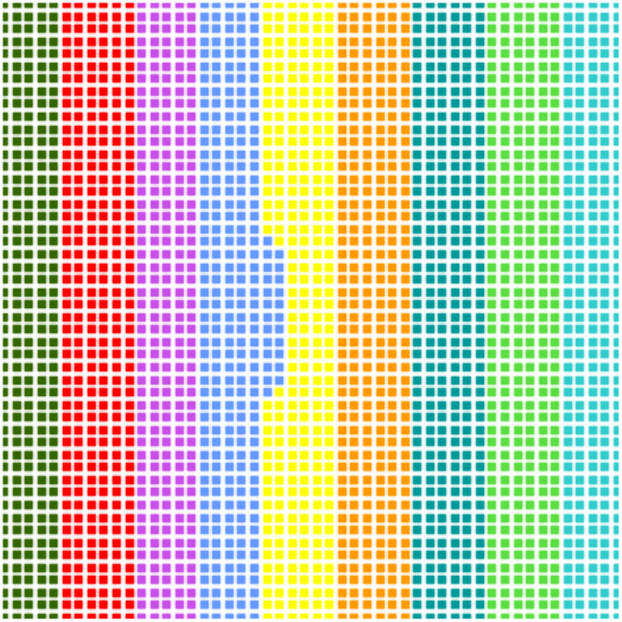
\includegraphics[width=0.6\linewidth]{images/results/m_k/with/2/partitioning}}
    \caption[short]{}
\end{subfigure}%
\begin{subfigure}{.33\textwidth}
    \centering
    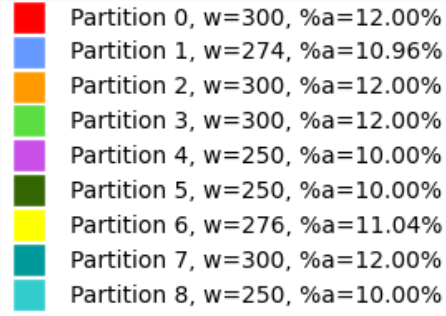
\includegraphics[width=0.9\linewidth]{images/results/m_k/with/2/results}
    \caption[short]{}
\end{subfigure}
\caption{Siatka $50$x$50$. Podział na $9$ partycji. Sumaryczna długość granic dla tego wyniku wynosi $402$.
Kryterium wyboru najlepszego rezultatu to najmniejsza różnica pomiędzy polem największej i najmniejszej partycji.}
\label{result:2}
\end{figure}

Siatka przedstawiona na rysunku \ref{result:2} jest trudnym przypadkiem, ponieważ nie daje znacznych możliwości na wyrównanie pól
w dalszych częściach algorytmu.
Wynik jest więc zależny od algorytmu LAM.
Aby otrzymać najlepszy rezultat musi on dobrze ustawić partycje od samego początku.
Dla tego przypadku nie da się otrzymać idealnie równego podziału, ale najlepszym rezultat będzie, gdy każda partycja będzie
w osobnym pionowym pasku.
Drugi obszar niepodzielny jest o jeden piksel węższy od pozostałych, dlatego w rezultacie partycjonowania pomiędzy partycją
$6$ a $1$ następuje wyrównanie pola.
Otrzymany rezultat jest najlepszym lub niemal najlepszym jaki można otrzymać.

\begin{figure}[h]
\centering
\begin{subfigure}{.33\textwidth}
    \centering
    \fbox{
\includegraphics[width=0.6\linewidth]{images/results/m_k/with/3/grid}}
    \caption[short]{}
\end{subfigure}%
\begin{subfigure}{.33\textwidth}
    \centering
    \fbox{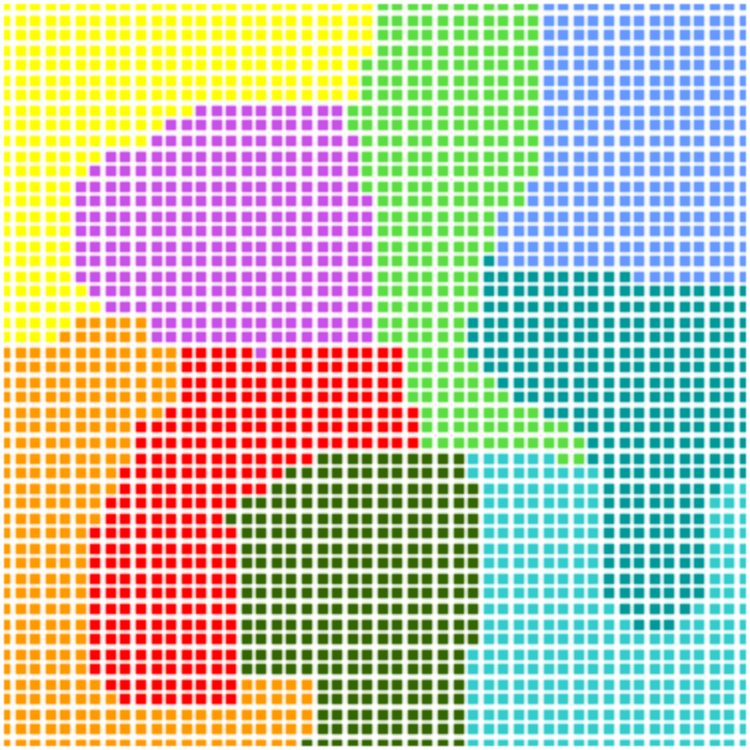
\includegraphics[width=0.6\linewidth]{images/results/m_k/with/3/partitioning}}
    \caption[short]{}
\end{subfigure}%
\begin{subfigure}{.33\textwidth}
    \centering
    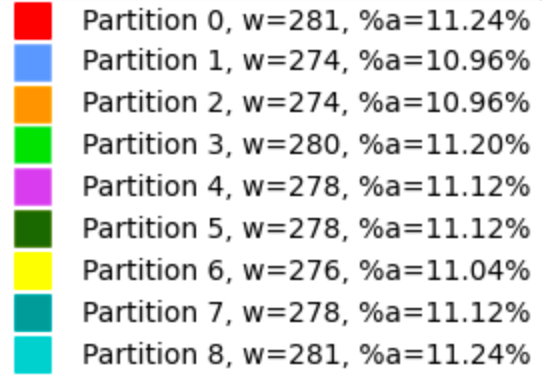
\includegraphics[width=0.9\linewidth]{images/results/m_k/with/3/results}
    \caption[short]{}
\end{subfigure}
\caption{Siatka $50$x$50$. Podział na $8$ partycji. Sumaryczna długość granic dla tego wyniku wynosi $313$.
Kryterium wyboru najlepszego rezultatu to najmniejsze odchylenie standardowe dla pól partycji.}
\label{result:3}
\end{figure}

Siatka partycjonowania na rysunku \ref{result:3} daje możliwość wymieniania się przez obszary wierzchołkami granicznymi,
jest to jednak znacznie utrudnione przez obszary niepodzielne.
Wyniki wybierane wedle kryterium najkrótszej długości granic dawały rezultaty z dużymi różnicami w kwestii pól partycji.
Rezultat daje niemal idealnie równe pola partycji, obszary są raczej zwarte.
Jest to dobry wynik.

\begin{figure}[h]
\centering
\begin{subfigure}{.33\textwidth}
    \centering
    \fbox{
\includegraphics[width=0.6\linewidth]{images/results/m_k/with/4/grid}}
    \caption[short]{}
\end{subfigure}%
\begin{subfigure}{.33\textwidth}
    \centering
    \fbox{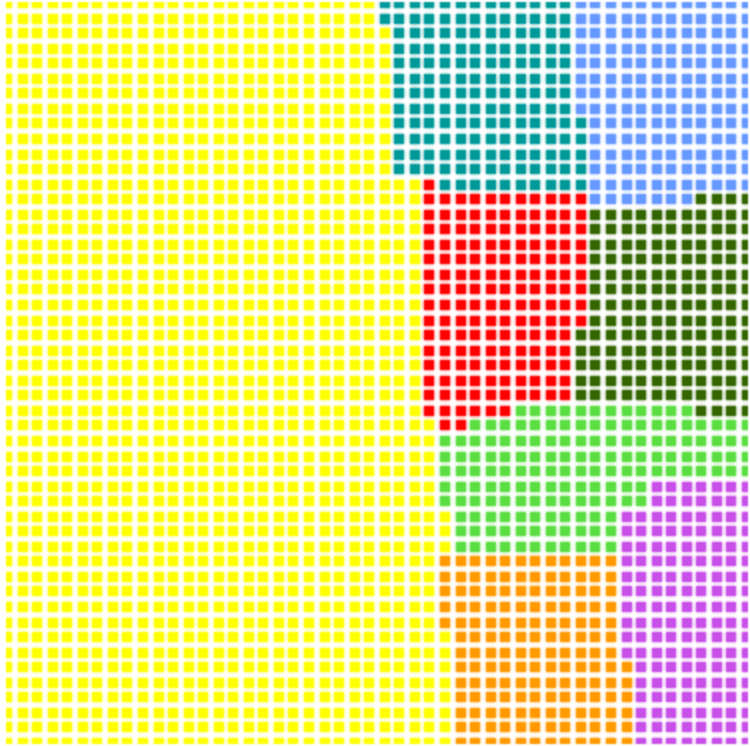
\includegraphics[width=0.6\linewidth]{images/results/m_k/with/4/partitioning}}
    \caption[short]{}
\end{subfigure}%
\begin{subfigure}{.33\textwidth}
    \centering
    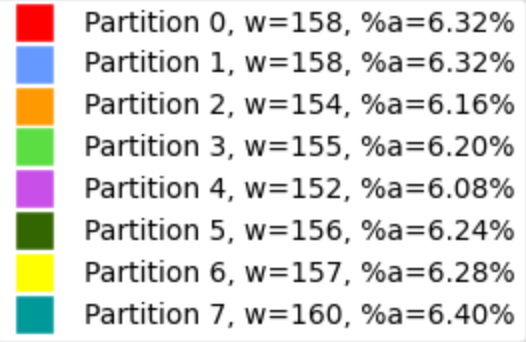
\includegraphics[width=0.9\linewidth]{images/results/m_k/with/4/results}
    \caption[short]{}
\end{subfigure}
\caption{Siatka $50$x$50$. Podział na $8$ partycji. Obszary wyłączone z obliczeń mapowane na wierzchołki z wagą $0$.
Sumaryczna długość granic dla tego wyniku wynosi $177$.
Wybór najlepszego rezultatu wedle kryterium najmniejszej długości granic.}
\label{result:4}
\end{figure}

\begin{figure}[h]
\centering
\begin{subfigure}{.33\textwidth}
    \centering
    \fbox{
\includegraphics[width=0.6\linewidth]{images/results/m_k/with/1/grid}}
    \caption[short]{}
\end{subfigure}%
\begin{subfigure}{.33\textwidth}
    \centering
    \fbox{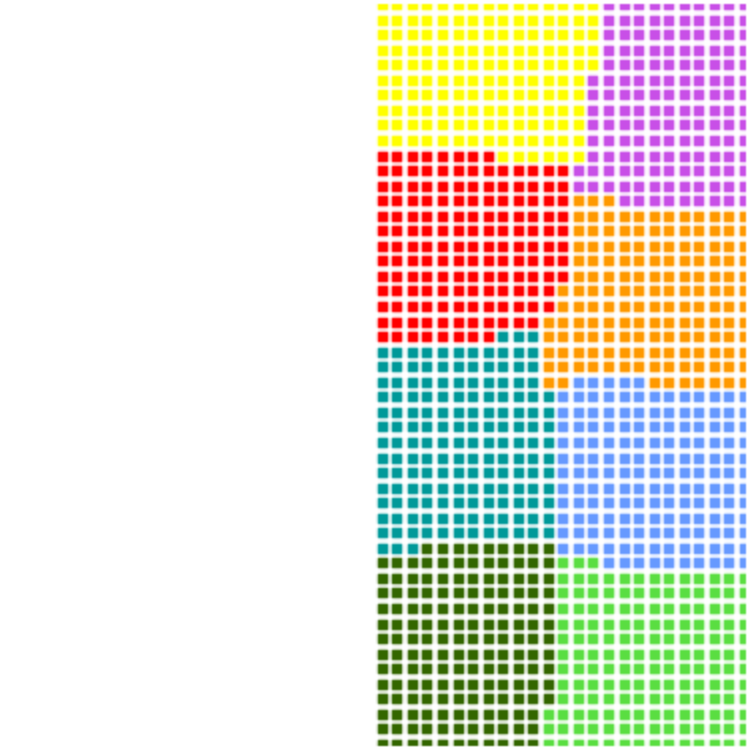
\includegraphics[width=0.6\linewidth]{images/results/m_k/with/1/partitioning}}
    \caption[short]{}
\end{subfigure}%
\begin{subfigure}{.33\textwidth}
    \centering
    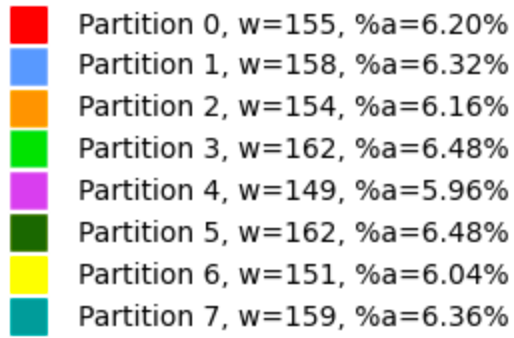
\includegraphics[width=0.9\linewidth]{images/results/m_k/with/1/results}
    \caption[short]{}
\end{subfigure}
\caption{Siatka $50$x$50$. Podział na $8$ partycji. Obszary wyłączone z obliczeń nie są mapowane na wierzchołki.
Sumaryczna długość granic dla tego wyniku wynosi $137$.
Wybór najlepszego rezultatu wedle kryterium najmniejszej długości granic.}
\label{result:1}
\end{figure}

Dla siatki przedstawionej na rysunku \ref{result:4} sprawdzane jest, czy algorytm bierze pod uwagę obszary wyłączone z obliczeń.
Na rezultacie widać, że wszystkie pola są niemal identyczne pod względem wagi.
Pole żółte urosło do dużych rozmiarów, jednak mimo to ma taką samą wagę jak pozostałe pola.
Algorytm poprawnie bierze pod uwagę obszary wyłączone z obliczeń.
Na rysunku \ref{result:1} przedstawiono partycjonowanie tej samej siatki, ale dla tego przypadku obszary wyłączone
z obliczeń nie są mapowane na wierzchołki w grafie.
W efekcie partycjonowanie trwa krócej, a długość granic jest znacznie mniejsza.

\vspace{8mm}
\begin{figure}[h]
\centering
\begin{subfigure}{.33\textwidth}
    \centering
    \fbox{
\includegraphics[width=0.6\linewidth]{images/results/m_k/with/5/grid}}
    \caption[short]{}
\end{subfigure}%
\begin{subfigure}{.33\textwidth}
    \centering
    \fbox{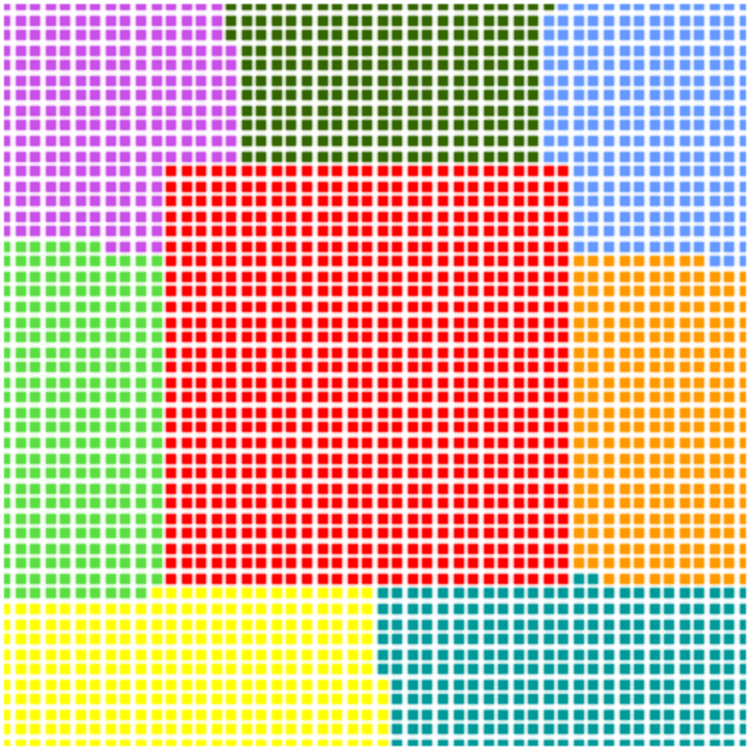
\includegraphics[width=0.6\linewidth]{images/results/m_k/with/5/partitioning}}
    \caption[short]{}
\end{subfigure}%
\begin{subfigure}{.33\textwidth}
    \centering
    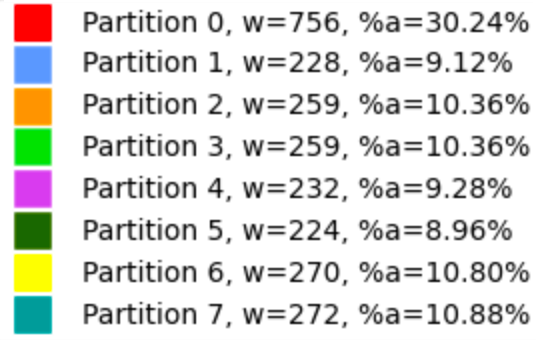
\includegraphics[width=0.9\linewidth]{images/results/m_k/with/5/results}
    \caption[short]{}
\end{subfigure}
\caption{Siatka $50$x$50$. Podział na $8$ partycji. Sumaryczna długość granic dla tego wyniku wynosi $196$.
Wybór najlepszego rezultatu wedle kryterium najmniejszej długości granic.}
\label{result:5}
\end{figure}

Dla siatki przedstawionej na rysunku \ref{result:5} sprawdzane jest działanie $discount$ dla algorytmu LAM.
Tego typu podziały są trudne dla algorytmu.
W rezultacie otrzymujemy podział, gdzie wszystkie obszary dookoła obszaru czerwonego mają niemal równe pola, co jest
najlepszym możliwym rezultatem dla tej siatki.
Nie są one idealnie równe, ponieważ podział był wybierany wedle kryterium długości granic.
Uznałem, że jest to lepsze kryterium, ponieważ wciąż algorytm ma całkiem dużą swobodę w kwestii optymalizacji granic i
pól partycji.

Rysunek \ref{result:6} oraz \ref{result:10} przedstawia partycjonowanie tej samej siatki.
Dla rysunku \ref{result:6} najlepszy rezultat został wybrany poprzez kryterium najmniejszego odchylenia standardowego
dla pól partycji, natomiast dla rysunku \ref{result:10} poprzez kryterium najmniejszej długość granic.
Widać jak różne podziały może tworzyć ten sam algorytm w zależności od początkowego ustawienia obszarów.
Dla rysunku \ref{result:6} otrzymaliśmy równiejsze pola, kosztem gorszej długości granic pomiędzy obszarami.
Na rysunku \ref{result:10} otrzymaliśmy krótsze granice, kosztem równości pól.
\begin{figure}[h]
\centering
\begin{subfigure}{.33\textwidth}
    \centering
    \fbox{
\includegraphics[width=0.6\linewidth]{images/results/m_k/with/6/grid}}
    \caption[short]{}
\end{subfigure}%
\begin{subfigure}{.33\textwidth}
    \centering
    \fbox{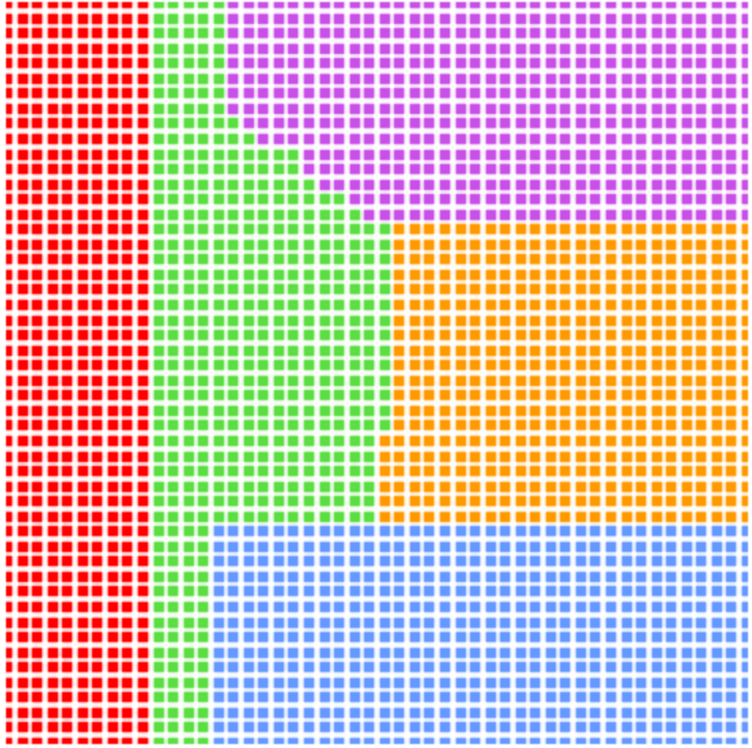
\includegraphics[width=0.6\linewidth]{images/results/m_k/with/6/partitioning}}
    \caption[short]{}
\end{subfigure}%
\begin{subfigure}{.33\textwidth}
    \centering
    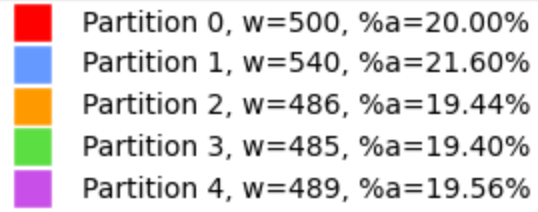
\includegraphics[width=0.9\linewidth]{images/results/m_k/with/6/results}
    \caption[short]{}
\end{subfigure}
\caption{Siatka $50$x$50$. Podział na $5$ partycji. Sumaryczna długość granic dla tego wyniku wynosi $172$.
Kryterium wyboru najlepszego rezultatu to najmniejsze odchylenie standardowe dla pól partycji.}
\label{result:6}
\end{figure}
\begin{figure}[h]
\centering
\begin{subfigure}{.33\textwidth}
    \centering
    \fbox{
\includegraphics[width=0.6\linewidth]{images/results/m_k/with/10/grid}}
    \caption[short]{}
\end{subfigure}%
\begin{subfigure}{.33\textwidth}
    \centering
    \fbox{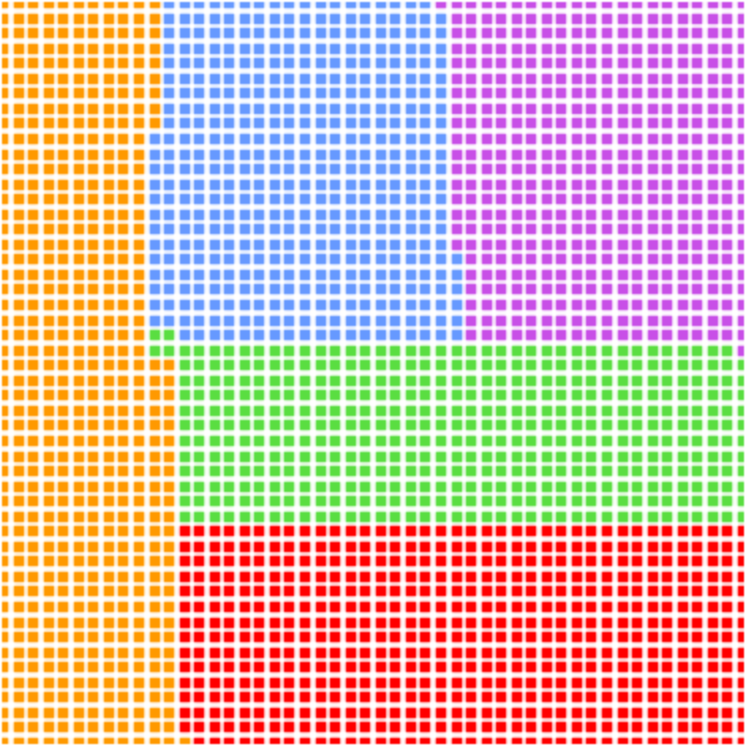
\includegraphics[width=0.6\linewidth]{images/results/m_k/with/10/partitioning}}
    \caption[short]{}
\end{subfigure}%
\begin{subfigure}{.33\textwidth}
    \centering
    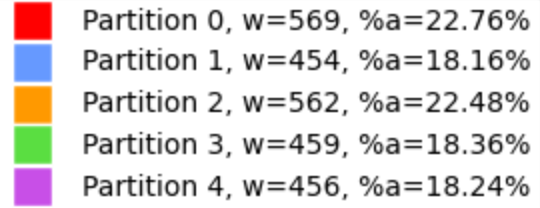
\includegraphics[width=0.9\linewidth]{images/results/m_k/with/10/results}
    \caption[short]{}
\end{subfigure}
\caption{Siatka $50$x$50$. Podział na $5$ partycji. Sumaryczna długość granic dla tego wyniku wynosi $159$.
Wybór najlepszego rezultatu wedle kryterium najmniejszej długości granic.}
\label{result:10}
\end{figure}

Rysunek \ref{result:7}, \ref{result:8} oraz \ref{result:9} przedstawia partycjonowanie tej samej siatki, odpowiednio na
$7$, $3$ oraz $10$ części.
Jest to bardzo trudna siatka do partycjonowania, ponieważ z racji na ułożenie obszarów niepodzielnych
nie pozwala na zbytnie minimalizowanie granic pomiędzy obszarami, a także wpływa na wielkość obszarów, ponieważ niektóre
obszary niepodzielne będą wymuszać większe partycje, niż powinny wyniknąć z podziału na zwykłej siatce tego
samego rozmiaru.
Pierwszy podział jest na $7$ części, ponieważ tyle jest białych i żółtych sfer na rysunku.
Algorytm próbuje wyrównywać pola na tyle, na ile jest to możliwe.
Widać, że partycje, które ze sobą sąsiadowały i miały możliwość wyrównania obszarów są w miarę tej samej wielkości.
Jest to na przykład partycja $6$ oraz $0$.
\begin{figure}[h]
\centering
\begin{subfigure}{.33\textwidth}
    \centering
    \fbox{
\includegraphics[width=0.6\linewidth]{images/results/m_k/with/7/grid}}
    \caption[short]{}
\end{subfigure}%
\begin{subfigure}{.33\textwidth}
    \centering
    \fbox{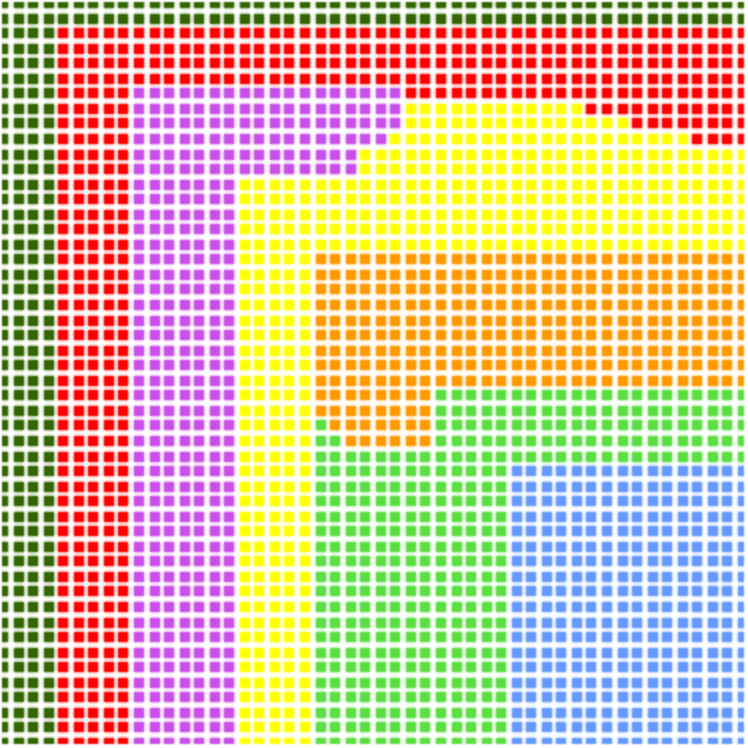
\includegraphics[width=0.6\linewidth]{images/results/m_k/with/7/partitioning}}
    \caption[short]{}
\end{subfigure}%
\begin{subfigure}{.33\textwidth}
    \centering
    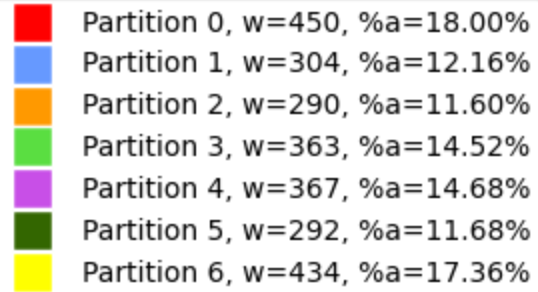
\includegraphics[width=0.9\linewidth]{images/results/m_k/with/7/results}
    \caption[short]{}
\end{subfigure}
\caption{Siatka $50$x$50$. Podział na $7$ partycji. Sumaryczna długość granic dla tego wyniku wynosi $369$.
Kryterium wyboru najlepszego rezultatu to najmniejsze odchylenie standardowe dla pól partycji.}
\label{result:7}
\end{figure}
\begin{figure}[h]
\centering
\begin{subfigure}{.33\textwidth}
    \centering
    \fbox{
\includegraphics[width=0.6\linewidth]{images/results/m_k/with/8/grid}}
    \caption[short]{}
\end{subfigure}%
\begin{subfigure}{.33\textwidth}
    \centering
    \fbox{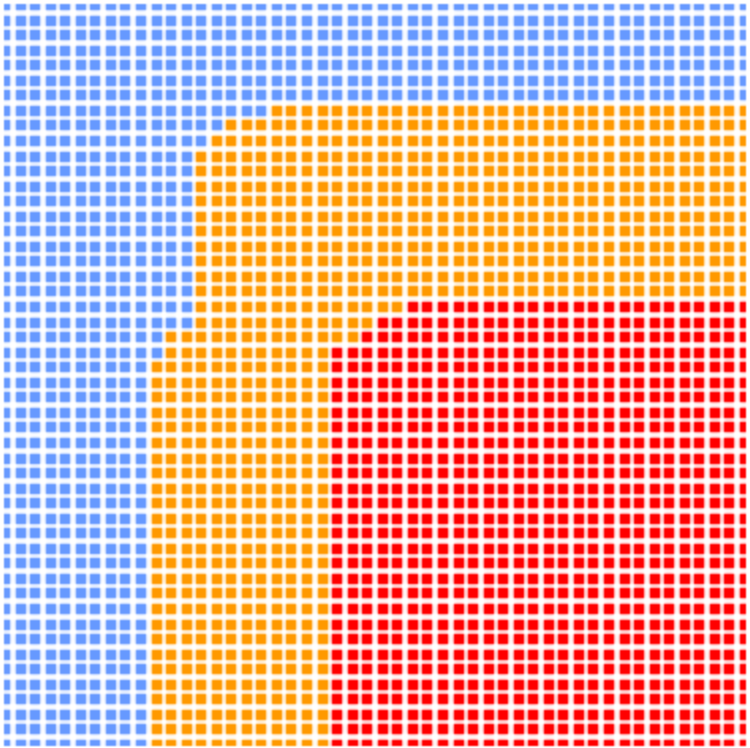
\includegraphics[width=0.6\linewidth]{images/results/m_k/with/8/partitioning}}
    \caption[short]{}
\end{subfigure}%
\begin{subfigure}{.33\textwidth}
    \centering
    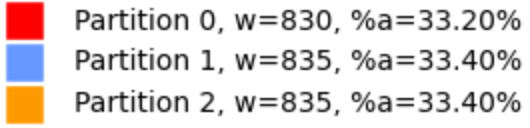
\includegraphics[width=0.9\linewidth]{images/results/m_k/with/8/results}
    \caption[short]{}
\end{subfigure}
\caption{Siatka $50$x$50$. Podział na $3$ partycje. Sumaryczna długość granic dla tego wyniku wynosi $141$.
Kryterium wyboru najlepszego rezultatu to najmniejsze odchylenie standardowe dla pól partycji.}
\label{result:8}
\end{figure}

\begin{figure}[h]
\centering
\begin{subfigure}{.33\textwidth}
    \centering
    \fbox{
\includegraphics[width=0.6\linewidth]{images/results/m_k/with/9/grid}}
    \caption[short]{}
\end{subfigure}%
\begin{subfigure}{.33\textwidth}
    \centering
    \fbox{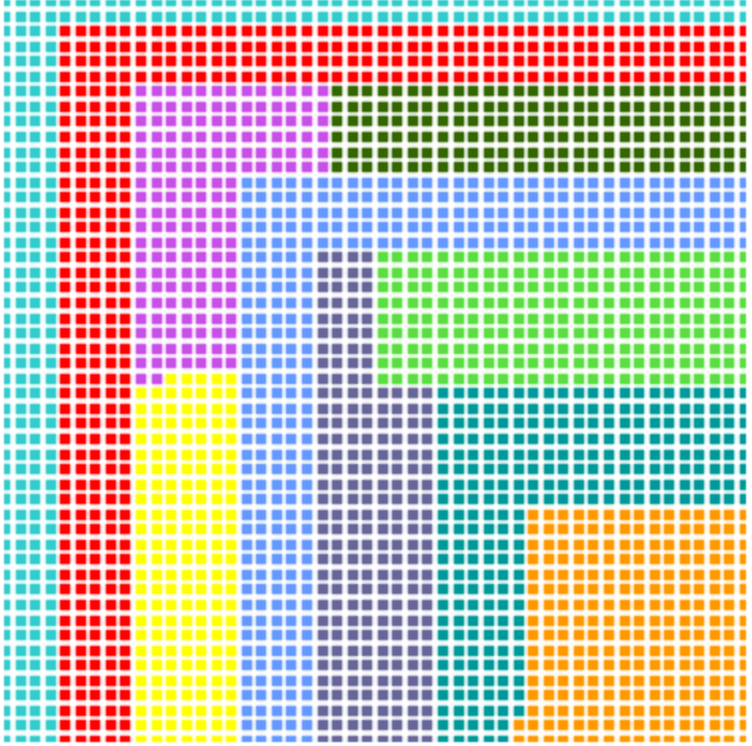
\includegraphics[width=0.6\linewidth]{images/results/m_k/with/9/partitioning}}
    \caption[short]{}
\end{subfigure}%
\begin{subfigure}{.33\textwidth}
    \centering
    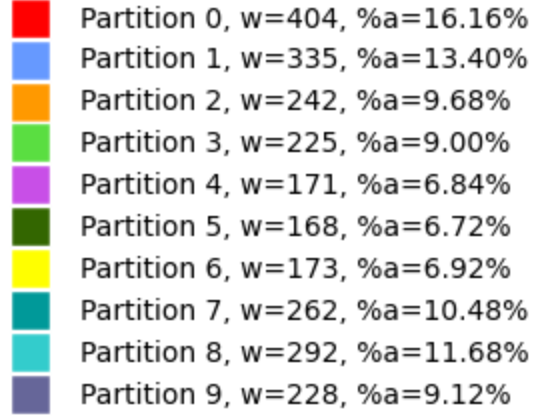
\includegraphics[width=0.9\linewidth]{images/results/m_k/with/9/results}
    \caption[short]{}
\end{subfigure}
\caption{Siatka $50$x$50$. Podział na $10$ partycji. Sumaryczna długość granic dla tego wyniku wynosi $417$.
Kryterium wyboru najlepszego rezultatu to najmniejsze odchylenie standardowe dla pól partycji.}
\label{result:9}
\end{figure}

Widać, że partycjonowanie na $3$ części na rysunku \ref{result:8} daje znacznie więcej swobody, w rezultacie
partycje są niemal identycznej wielkości.
Ustawienie obszarów niepodzielnych motywuje nadal ułożenie partycji i zwiększa długość granic.
Partycjonowanie przedstawione na rysunku \ref{result:9} to bardziej ekstremalna wersja partycjonowania na rysunku \ref{result:7}.
Partycje, które miały możliwość wyrównania pola między sobą, jak partycje $6$, $4$ oraz $5$,
mają praktycznie identyczne pola.
Analizując ten rysunek trudno jest zaproponować lepsze początkowe ułożenie obszarów w celu późniejszej, lepszej optymalizacji
pól obszarów.
Algorytm bardzo dobrze radzi sobie z tym trudnym przypadkiem.

\vspace{4mm}

Rysunek \ref{result:11} oraz \ref{result:12} pokazuje bardzo podobną sytuację jak dla rysunku \ref{result:6} oraz
\ref{result:10}.
Dla rysunku \ref{result:11} otrzymaliśmy równiejsze pola, kosztem gorszej długości granic pomiędzy obszarami.
Na rysunku \ref{result:12} otrzymaliśmy krótsze granice, kosztem równości pól.
Różnicą w tym wypadku jest to, że na raz na siatce pojawiają się zarówno obszary wyłączone z obliczeń jak i
obszary niepodzielne.
Algorytm bardzo dobrze radzi sobie z uwzględnieniem obydwu, otrzymuje krótkie granice oraz niemal równe obszary.
\begin{figure}[h]
\centering
\begin{subfigure}{.33\textwidth}
    \centering
    \fbox{
\includegraphics[width=0.6\linewidth]{images/results/m_k/with/11/grid}}
    \caption[short]{}
\end{subfigure}%
\begin{subfigure}{.33\textwidth}
    \centering
    \fbox{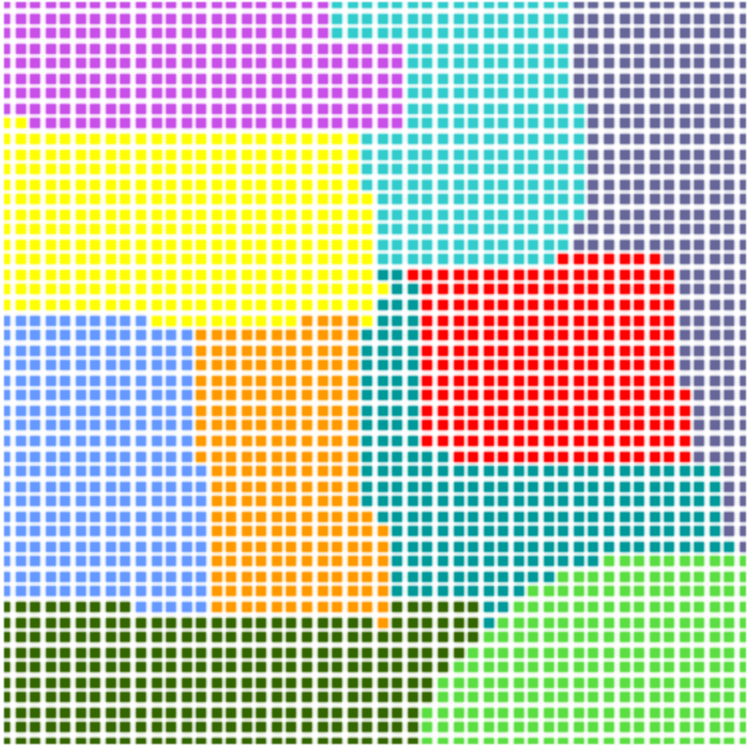
\includegraphics[width=0.6\linewidth]{images/results/m_k/with/11/partitioning}}
    \caption[short]{}
\end{subfigure}%
\begin{subfigure}{.33\textwidth}
    \centering
    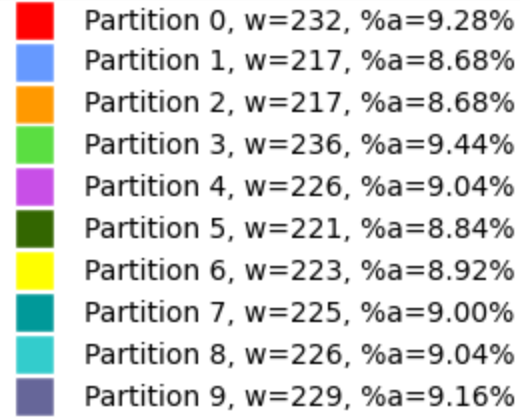
\includegraphics[width=0.9\linewidth]{images/results/m_k/with/11/results}
    \caption[short]{}
\end{subfigure}
\caption{Siatka $50$x$50$. Podział na $10$ partycji.
Obszary wyłączone z obliczeń mapowane na wierzchołki z wagą $0$.
Sumaryczna długość granic dla tego wyniku wynosi $295$.
Kryterium wyboru najlepszego rezultatu to najmniejsze odchylenie standardowe dla pól partycji.}
\label{result:11}
\end{figure}
\begin{figure}[h]
\centering
\begin{subfigure}{.33\textwidth}
    \centering
    \fbox{
\includegraphics[width=0.6\linewidth]{images/results/m_k/with/12/grid}}
    \caption[short]{}
\end{subfigure}%
\begin{subfigure}{.33\textwidth}
    \centering
    \fbox{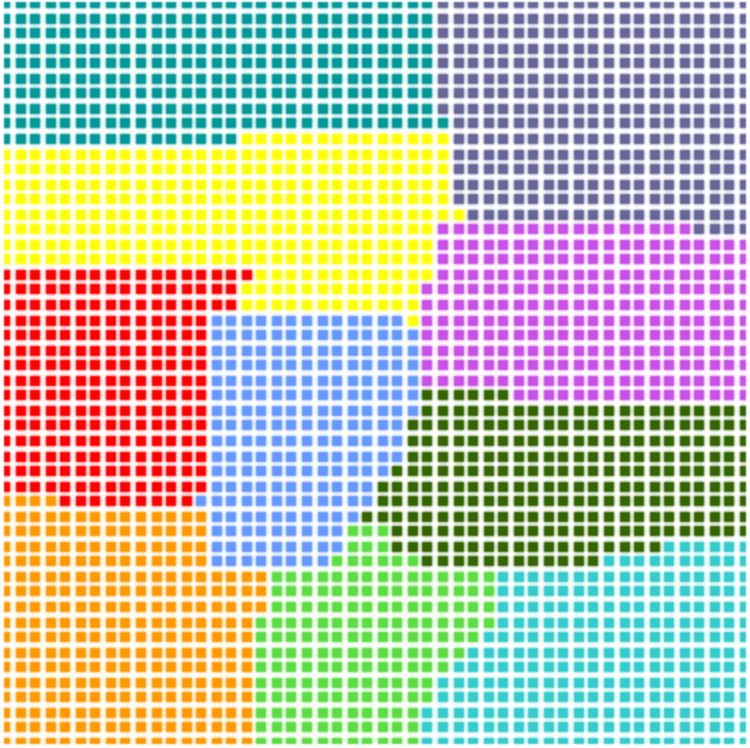
\includegraphics[width=0.6\linewidth]{images/results/m_k/with/12/partitioning}}
    \caption[short]{}
\end{subfigure}%
\begin{subfigure}{.33\textwidth}
    \centering
    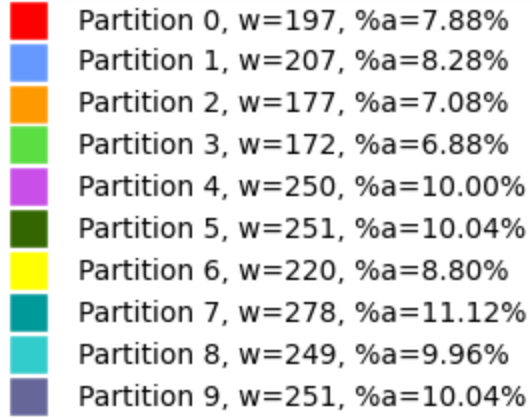
\includegraphics[width=0.9\linewidth]{images/results/m_k/with/12/results}
    \caption[short]{}
\end{subfigure}
\caption{Siatka $50$x$50$. Podział na $10$ partycji.
Obszary wyłączone z obliczeń mapowane na wierzchołki z wagą $0$.
Sumaryczna długość granic dla tego wyniku wynosi $261$.
Wybór najlepszego rezultatu wedle kryterium najmniejszej długości granic.}
\label{result:12}
\end{figure}
\FloatBarrier
\begin{figure}[h]
\centering
\begin{subfigure}{.33\textwidth}
    \centering
    \fbox{
\includegraphics[width=0.6\linewidth]{images/results/m_k/with/14/grid}}
    \caption[short]{}
\end{subfigure}%
\begin{subfigure}{.33\textwidth}
    \centering
    \fbox{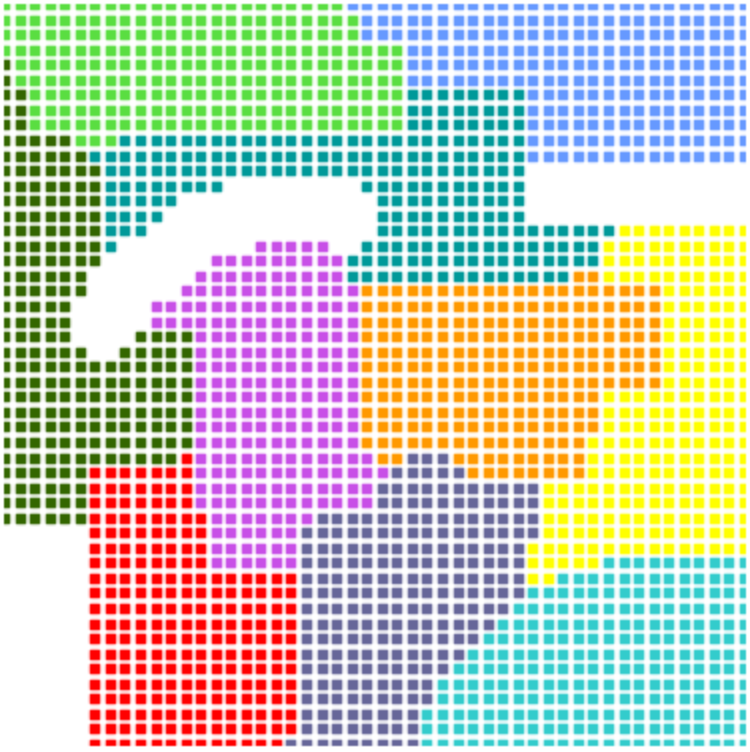
\includegraphics[width=0.6\linewidth]{images/results/m_k/with/14/partitioning}}
    \caption[short]{}
\end{subfigure}%
\begin{subfigure}{.33\textwidth}
    \centering
    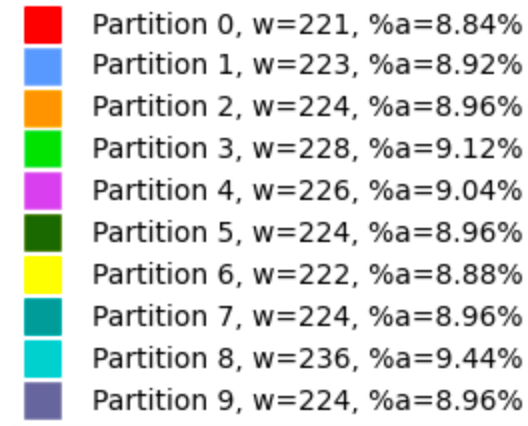
\includegraphics[width=0.9\linewidth]{images/results/m_k/with/14/results}
    \caption[short]{}
\end{subfigure}
\caption{Siatka $50$x$50$. Podział na 10 partycji.
Obszary wyłączone z obliczeń nie są mapowane na wierzchołki.
Sumaryczna długość granic dla tego wyniku wynosi $252$.
Kryterium wyboru najlepszego rezultatu to najmniejsze odchylenie standardowe dla pól partycji.}
\label{result:14}
\end{figure}
\begin{figure}[h]
\centering
\begin{subfigure}{.33\textwidth}
    \centering
    \fbox{
\includegraphics[width=0.6\linewidth]{images/results/m_k/with/13/grid}}
    \caption[short]{}
\end{subfigure}%
\begin{subfigure}{.33\textwidth}
    \centering
    \fbox{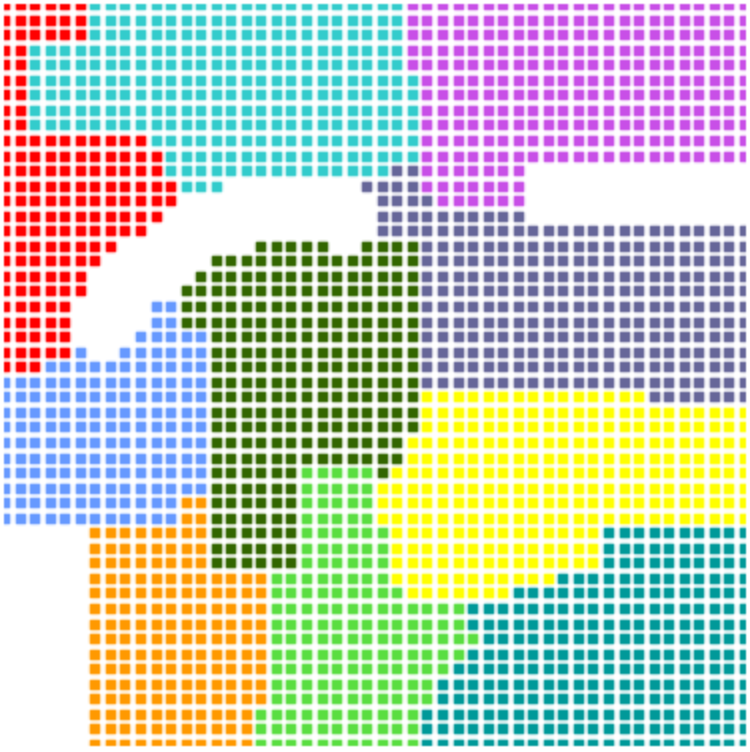
\includegraphics[width=0.6\linewidth]{images/results/m_k/with/13/partitioning}}
    \caption[short]{}
\end{subfigure}%
\begin{subfigure}{.33\textwidth}
    \centering
    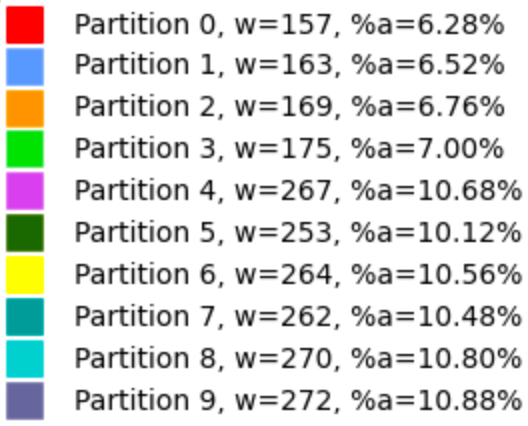
\includegraphics[width=0.9\linewidth]{images/results/m_k/with/13/results}
    \caption[short]{}
\end{subfigure}
\caption{Siatka $50$x$50$. Podział na 10 partycji.
Obszary wyłączone z obliczeń nie są mapowane na wierzchołki.
Sumaryczna długość granic dla tego wyniku wynosi $221$.
Wybór najlepszego rezultatu wedle kryterium najmniejszej długości granic.}
\label{result:13}
\end{figure}
Rysunek \ref{result:13} oraz \ref{result:14} prezentują partycjonowanie tej samej siatki, ale z użyciem wariantu algorytmu
gdzie obszary wyłączone z obliczeń nie są mapowane na wierzchołki.
W efekcie dla obydwu kryteriów wyboru najlepszego partycjonowania otrzymujemy mniejszą długość granic.
Do tej pory dla wszystkich przykładów nietworzenie wierzchołków w miejsce obszarów wyłączonych z obliczeń
zwracało lepsze rezultaty i ten trend utrzyma się do samego końca.
Dodatkowo dalej pokażę, że jeśli są one duże i nie są skupione w jednych miejscach siatki to są bardzo
problematyczne dla algorytmu LAM, a także znaczenie wydłużają czas partycjonowania.
Zawsze szybszym, efektywniejszym wyjściem jest skorzystanie z opcji usunięcia ich z siatki.
\FloatBarrier

